\documentclass[aspectratio=169, 12pt]{beamer}
\usetheme[progressbar=frametitle, numbering=fraction, block=fill]{metropolis}

\usepackage{amsmath, amssymb}
\usepackage{graphicx}
\usepackage{booktabs}
\usepackage{xcolor}

% -- colours ----------------------------------------------------------
\definecolor{accent}{RGB}{0,120,200}
\definecolor{darkbg}{RGB}{35,40,50}
\definecolor{softgray}{RGB}{140,145,155}
\definecolor{okgreen}{RGB}{50,180,90}
\definecolor{warnred}{RGB}{220,80,60}

\setbeamercolor{frametitle}{bg=darkbg, fg=white}
\setbeamercolor{progress bar}{fg=accent}
\setbeamercolor{alerted text}{fg=accent}

% -- fonts ------------------------------------------------------------
\setbeamerfont{title}{size=\Large, series=\bfseries}
\setbeamerfont{frametitle}{size=\large}

\setbeamertemplate{navigation symbols}{}

% -- metadata ---------------------------------------------------------
\title{Backstepping Swing-Up and Stabilization of the Acrobot}
\subtitle{Project~3 --- Advanced Control Methods}
\author{\footnotesize Mariya Lezina\enspace\textbullet\enspace Safina Gulyamova\enspace\textbullet\enspace Hajira Amjad\enspace\textbullet\enspace Ilya Mikhalchuk\enspace\textbullet\enspace Mikhail Sannikov}
\institute{Skoltech, 2026}
\date{}

\begin{document}

% =====================================================================
%  SLIDE 1 -- Title
% =====================================================================
\begin{frame}[plain]
  \maketitle
\end{frame}

\note{%
Hello, we are team [NAME]. This is our third project: backstepping control
for the acrobot with actuator dynamics.
}


% =====================================================================
%  SLIDE 2 -- The Acrobot System
% =====================================================================
\begin{frame}{The Acrobot with Actuator Dynamics}
\footnotesize
\begin{columns}[T]
\begin{column}{0.45\textwidth}
  \textbf{Same underactuated acrobot, new input path.}
  \begin{itemize}
    \item Shoulder joint is \alert{unactuated}
    \item Elbow torque $\tau_2$ is an \alert{actuator state}
    \item Command $u$ is filtered:
      $T_a\dot{\tau}_2 = u-\tau_2$
    \item $T_a = 0.005$~s,\quad $|u| \le 50$~N\,m
    \item State:
      $x = [q_1, q_2, \dot{q}_1, \dot{q}_2, \tau_2]^\top$
    \item Goal: swing up and stabilize using only $u$
  \end{itemize}
\end{column}
\begin{column}{0.26\textwidth}
  \centering
  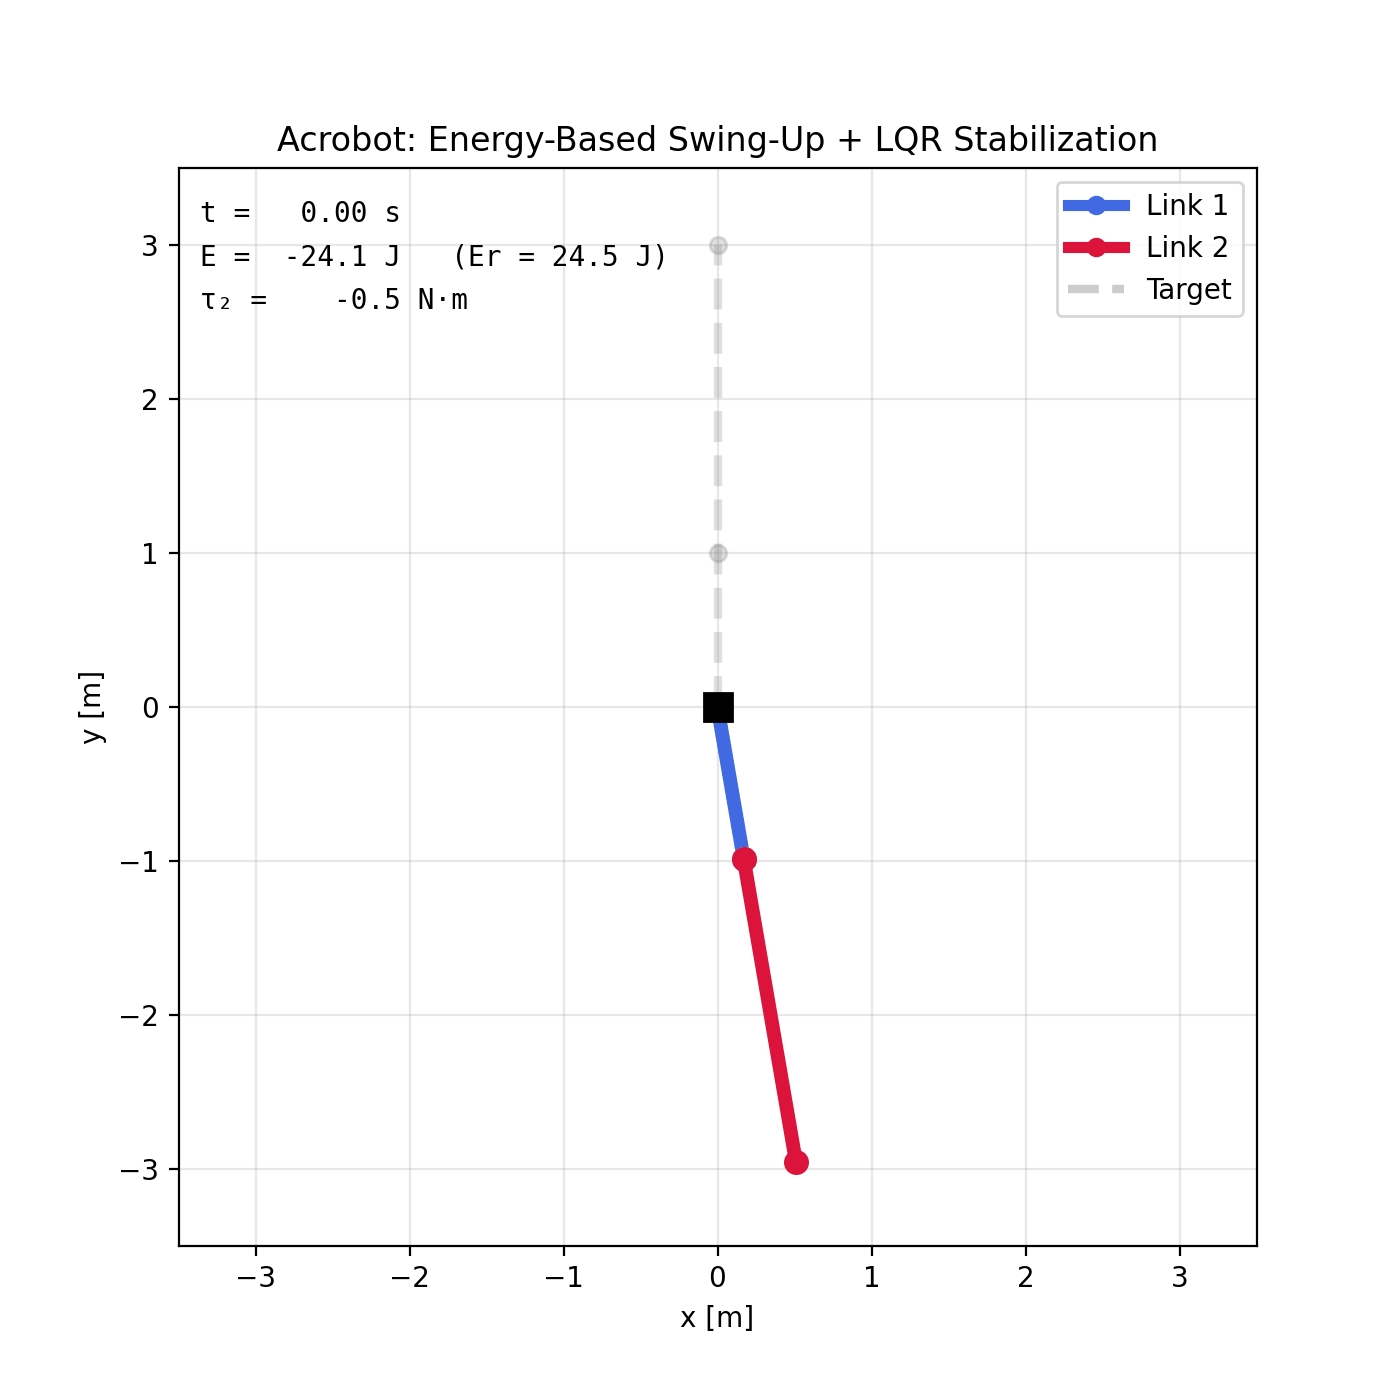
\includegraphics[height=0.54\textheight]{figures/acrobot_frame_hanging.png}\\[2pt]
  {\small Hanging (stable)\\$q_1 = -\tfrac{\pi}{2}$}
\end{column}
\begin{column}{0.26\textwidth}
  \centering
  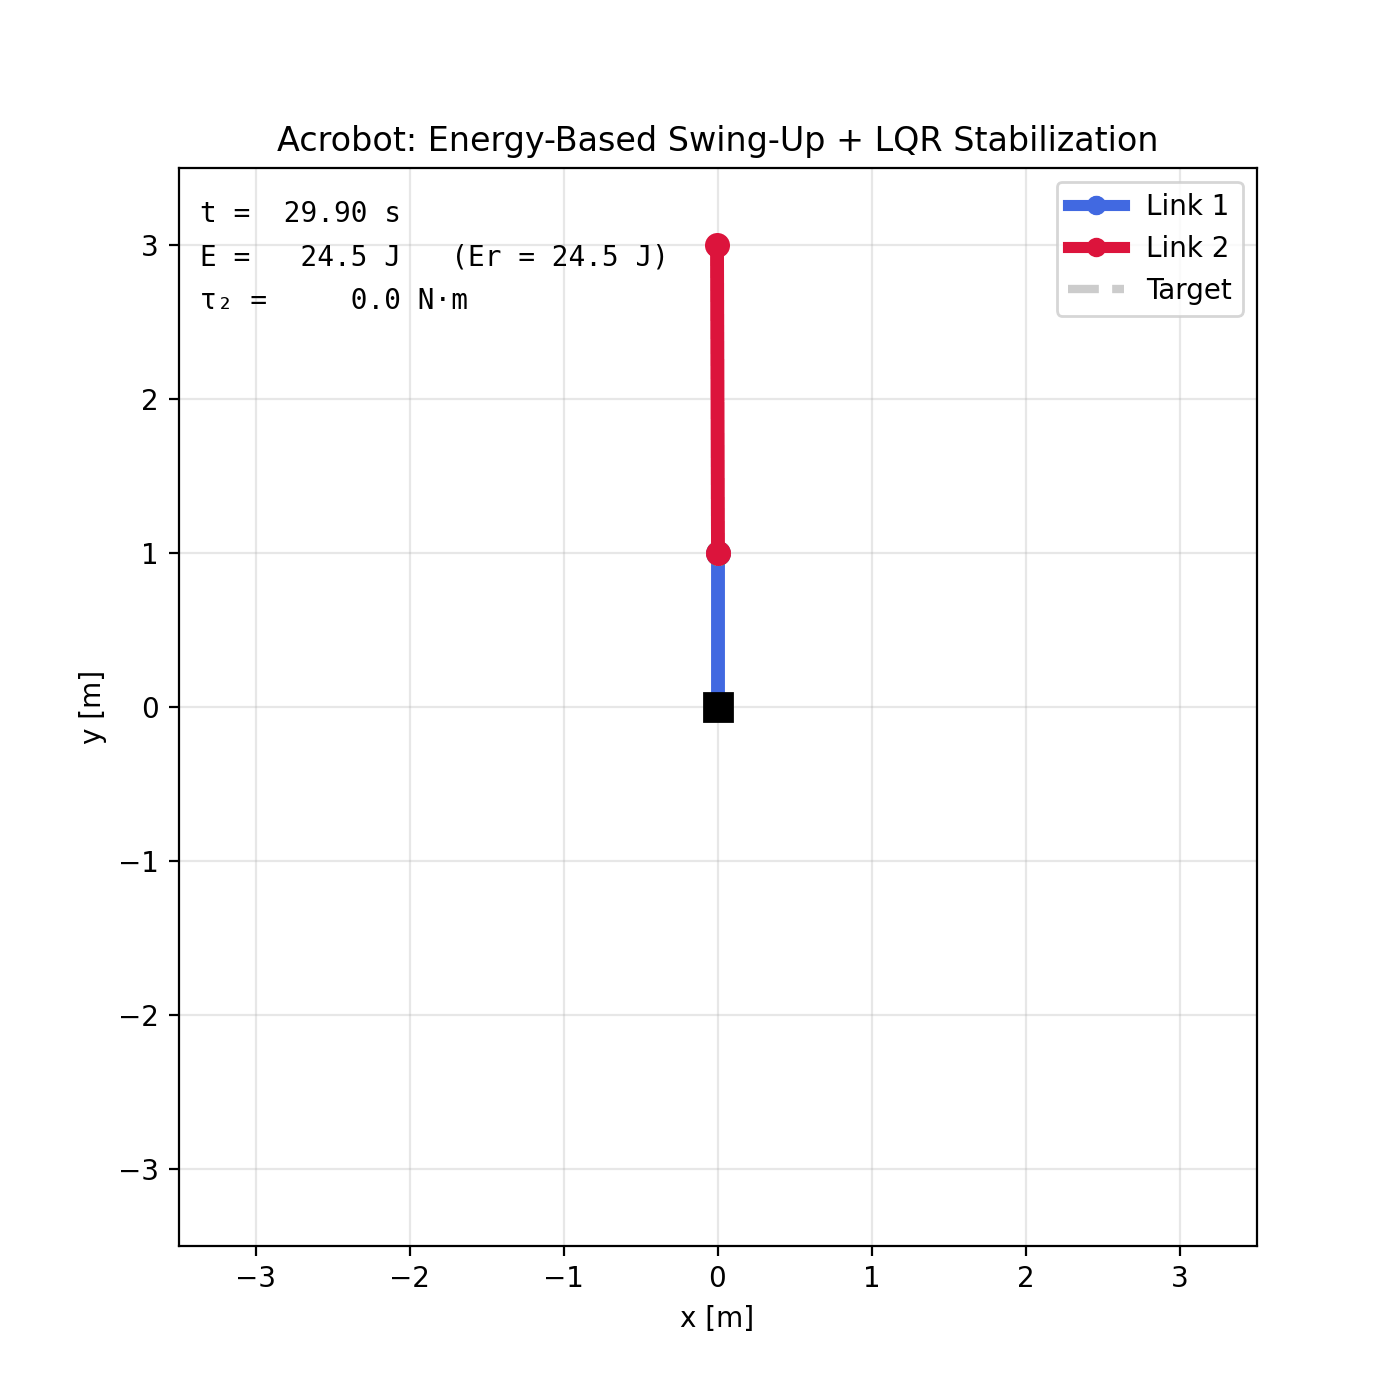
\includegraphics[height=0.54\textheight]{figures/acrobot_frame_final.png}\\[2pt]
  {\small Upright (unstable)\\$q_1 = +\tfrac{\pi}{2}$}
\end{column}
\end{columns}
\end{frame}

\note{%
The mechanical acrobot is the same two-link system from Project 1.
The top joint is passive, and the only physical torque acts at the elbow.

The difference is that we do not command that elbow torque directly anymore.
We command u, and the actuator output tau-two follows u through a first-order
lag with time constant T-a.

So the state has one extra coordinate: tau-two itself.
The control problem is to swing up and stabilize the acrobot while compensating
for this actuator lag.
}


% =====================================================================
%  SLIDE 3 -- Equations of Motion
% =====================================================================
\begin{frame}{Equations of Motion}
\small
\[
  M(q)\,\ddot{q} + C(q,\dot{q})\,\dot{q} + G(q)
  = \begin{bmatrix} 0 \\ \tau_2 \end{bmatrix},
  \qquad
  T_a\,\dot{\tau}_2 = u - \tau_2
\]

\begin{columns}[T]
\begin{column}{0.48\textwidth}
  \textbf{Mechanical subsystem:}
  {\footnotesize
  \[
    M = \begin{bmatrix}
      \alpha_1 + \alpha_2 + 2\alpha_3 \cos q_2
        & \alpha_2 + \alpha_3 \cos q_2 \\
      \alpha_2 + \alpha_3 \cos q_2
        & \alpha_2
    \end{bmatrix}
  \]
  \[
    C\dot{q} = \alpha_3 \sin q_2
    \begin{bmatrix}
      -2\dot{q}_1 \dot{q}_2 - \dot{q}_2^2 \\
      \dot{q}_1^2
    \end{bmatrix}
  \]
  \[
    G = \begin{bmatrix}
      \beta_1 \cos q_1 + \beta_2 \cos(q_1{+}q_2) \\
      \beta_2 \cos(q_1{+}q_2)
    \end{bmatrix}
  \]
  }
\end{column}
\begin{column}{0.48\textwidth}
  \textbf{Lumped parameters:}
  {\footnotesize
  \begin{align*}
    \alpha_1 &= m_1 l_{c1}^2 + m_2 l_1^2 + I_1 \\
    \alpha_2 &= m_2 l_{c2}^2 + I_2 \\
    \alpha_3 &= m_2\, l_1\, l_{c2} \\[6pt]
    \beta_1  &= (m_1 l_{c1} + m_2 l_1)\,g \\
    \beta_2  &= m_2\, l_{c2}\, g
  \end{align*}
  }

  \smallskip
  The actuator adds one state but does not change $M$, $C$, or $G$.
\end{column}
\end{columns}
\end{frame}

\note{%
The mechanical equations are unchanged from Project 1.
The mass matrix, Coriolis vector, and gravity vector are the same.

The new row is the actuator equation.
Tau-two is the torque that the mechanical system actually receives, and u is
the command we choose.
This distinction is the reason we need backstepping.
}


% =====================================================================
%  SLIDE 4 -- Backstepping Idea
% =====================================================================
\begin{frame}{Backstepping Idea}
\small
\begin{columns}[T]
\begin{column}{0.52\textwidth}
  \textbf{Reuse Project~1 as the outer loop.}
  \[
    V_0 = \tfrac{1}{2}(E - E_r)^2
             + \tfrac{1}{2}\,k_D\,\dot{q}_2^2
             + \tfrac{1}{2}\,k_P\,q_2^2
  \]

  If the elbow torque were direct, Project~1 would choose $\tau_2^\ast$
  so that
  \[
    \dot{V}_0 = -k_V\,\dot{q}_2^2 \le 0.
  \]

  In Project~3, $\tau_2^\ast$ becomes a \alert{virtual control}:\\
  the desired actuator output, not the command.

  \smallskip
  \textbf{Backstepping task:} make $\tau_2(t)$ track
  $\tau_2^\ast(q,\dot{q})$ fast enough for the outer energy proof.
\end{column}
\begin{column}{0.46\textwidth}
  \centering
  
\includegraphics[width=0.95\textwidth]{figures/energy.png}

  \smallskip
  {\footnotesize\color{softgray}
  The same target energy $E_r = 24.5$~J is used, but actuator lag must be
  compensated before LQR can catch the upright pass.}
\end{column}
\end{columns}
\end{frame}

\note{%
Backstepping starts from the controller we already know.
Project 1 gives us a torque tau-two-star that would make the energy Lyapunov
function decrease if it were applied directly.

With actuator dynamics, tau-two-star is not the command anymore.
It is the virtual control: the torque we want the actuator output to track.

The inner-loop problem is therefore to choose u so that the actual tau-two
follows tau-two-star with a small tracking error.
}


% =====================================================================
%  SLIDE 5 -- Backstepping Control Law
% =====================================================================
\begin{frame}{Backstepping Control Law}
\small
Project~1's energy-shaping torque is reused as the virtual control
$\tau_2^\ast(q,\dot q)$; the command $u$ makes the actuator output track it.

\medskip
\begin{columns}[T]
\begin{column}{0.48\textwidth}
  \footnotesize
  \textbf{Inner tracking error:}
  \[
    z = \tau_2 - \tau_2^\ast
  \]

  \textbf{Command law:}
  \[
    \boxed{u = \tau_2^\ast
      + T_a\,\dot{\tau}_2^\ast
      - k_z T_a z}
  \]

  \textbf{Resulting error dynamics:}
  \[
    \dot{z} = -\Bigl(\tfrac{1}{T_a}+k_z\Bigr)z
  \]
\end{column}
\begin{column}{0.48\textwidth}
  \footnotesize
  \textbf{Chain-rule feedforward:}
  \[
    \dot{\tau}_2^\ast =
      \sum_{k=1}^{4}
      \frac{\partial \tau_2^\ast}{\partial x_{m,k}}\dot{x}_{m,k}
  \]
  The mechanical acceleration uses the \alert{actual} $\tau_2$, and the
  gradient is evaluated by central finite differences.

  \smallskip
  \textbf{Gains:}
  \[
    k_D = 35.8,\quad k_P = 61.2,\quad
    k_V = 66.3,\quad k_z = 25
  \]
  Inner time constant: $\approx 4.4$~ms.
\end{column}
\end{columns}
\end{frame}

\note{%
The virtual torque is exactly the Project 1 energy-shaping formula.
We define z as the difference between actual torque and desired virtual torque.

The command has three terms.
The first term asks for the desired torque.
The second term is feedforward: it predicts where tau-two-star is going after
one actuator time constant.
The third term is feedback on the actuator tracking error.

After substitution into the actuator equation, z follows a stable first-order
linear equation.
With our numbers, the tracking error decays with a time constant of about
four point four milliseconds.
}


% =====================================================================
%  SLIDE 6 -- LQR Stabilization
% =====================================================================
\begin{frame}{LQR Stabilization \& Controller Switching}
\footnotesize
\begin{columns}[T]
\begin{column}{0.50\textwidth}
  \textbf{Augmented Lyapunov function:}
  \[
    V_3 = V_0 + \tfrac{1}{2}z^2
  \]
  The inner loop makes $z$ decay exponentially, so the outer energy
  controller recovers the Project~1 swing-up behavior.

  \medskip
  \textbf{Phase~2 --- LQR at the upright:}\\[3pt]
  Use the Project~1 mechanical LQR and add actuator damping:
  \[
    u = -K
    \begin{bmatrix}
      e_{q_1} & q_2 & \dot{q}_1 & \dot{q}_2 & \tau_2
    \end{bmatrix}^{\top}
  \]
  {\scriptsize
  \[
    K =
    \begin{bmatrix}
      -238.6 & -95.6 & -103.0 & -48.6 & 1.0
    \end{bmatrix}
  \]
  }
\end{column}
\begin{column}{0.47\textwidth}
  \textbf{Switching strategy:}
  \begin{enumerate}\setlength\itemsep{2pt}
    \item Backstepping swing-up runs.
    \item Monitor mechanical error only:\\
          $\|e\|_w = |e_{q_1}|{+}|q_2|{+}0.1|\dot{q}_1|{+}0.1|\dot{q}_2|$
    \item $\|e\|_w < 0.04 \;\Rightarrow$ \alert{switch to LQR}.
    \item One-way switch until $t = 30$~s.
  \end{enumerate}

  \smallskip
  Switch occurs at $t \approx 7.8$~s.

  \smallskip
  \centering
  
\includegraphics[width=0.88\textwidth]{figures/control_signal.png}
\end{column}
\end{columns}
\end{frame}

\note{%
For the stability argument, we add one extra term to the Lyapunov function:
one half z squared.
The backstepping law drives this new error to zero quickly, so the mechanical
part behaves like the Project 1 energy controller.

Near the top, we still switch to LQR.
In practice, the full 5D Riccati gain was too aggressive under command
saturation, so we use the Project 1 mechanical LQR and add a small damping
gain on the actuator state.

The switch condition is the same weighted mechanical error as before, with
threshold zero point zero four.
}


% =====================================================================
%  SLIDE 7 -- Code Structure
% =====================================================================
\begin{frame}{Implementation}
\footnotesize
\begin{columns}[T]
\begin{column}{0.43\textwidth}
  \textbf{Project structure:}

  \smallskip
  {\scriptsize
  \begin{tabular}{@{}l@{\;\;---\;\;}l@{}}
    \texttt{configs/params.py}    & params \\
    \texttt{src/system.py}        & 5D dynamics \\
    \texttt{src/controller.py}    & controllers \\
    \texttt{src/simulation.py}    & switching ODE \\
    \texttt{src/visualization.py} & plots \\
    \texttt{src/animation.py}     & GIF \\
    \texttt{src/main.py}          & entry point \\
  \end{tabular}
  }

  \medskip
  \textbf{Reproduce:}\\[2pt]
  {\scriptsize
  \texttt{pip install -r requirements.txt}\\
  \texttt{python -m src.main}\\
  \texttt{python -m src.main --no-anim}\\[2pt]
  }
  Deps: \texttt{numpy}, \texttt{scipy}, \texttt{matplotlib}.
\end{column}
\begin{column}{0.53\textwidth}
  \textbf{Algorithm:}
  {\scriptsize
  \begin{enumerate}\setlength\itemsep{1pt}
    \item Build 5D plant: $T_a\dot{\tau}_2 = u-\tau_2$
    \item Verify inherited $k_D$ solvability bound
    \item Compute Project~1 virtual torque $\tau_2^\ast$
    \item Estimate $\dot{\tau}_2^\ast$ by chain rule
    \item Command $u=\tau_2^\ast+T_a\dot{\tau}_2^\ast-k_zT_az$
    \item Switch to LQR when $\|e\|_w < 0.04$
    \item Generate plots, comparisons, and animation
  \end{enumerate}
  }

\end{column}
\end{columns}
\end{frame}

\note{%
The implementation keeps the same modular structure as Project 1.
The system file contains the 5D dynamics, including actuator lag.
The controller file contains the virtual torque, backstepping command, LQR,
and the Project 1 baseline used for comparison.

The main script runs the backstepping simulation, runs the naive Project 1
baseline on the same actuator-lag plant, and then generates the plots and
animation.
}


% =====================================================================
%  SLIDE 8 -- Animation
% =====================================================================
{
\setbeamercolor{background canvas}{bg=darkbg}
\begin{frame}[plain]
  \centering
  \vspace{0.5cm}
  {\Large\color{white}\bfseries Animation}

  \vspace{0.3cm}
  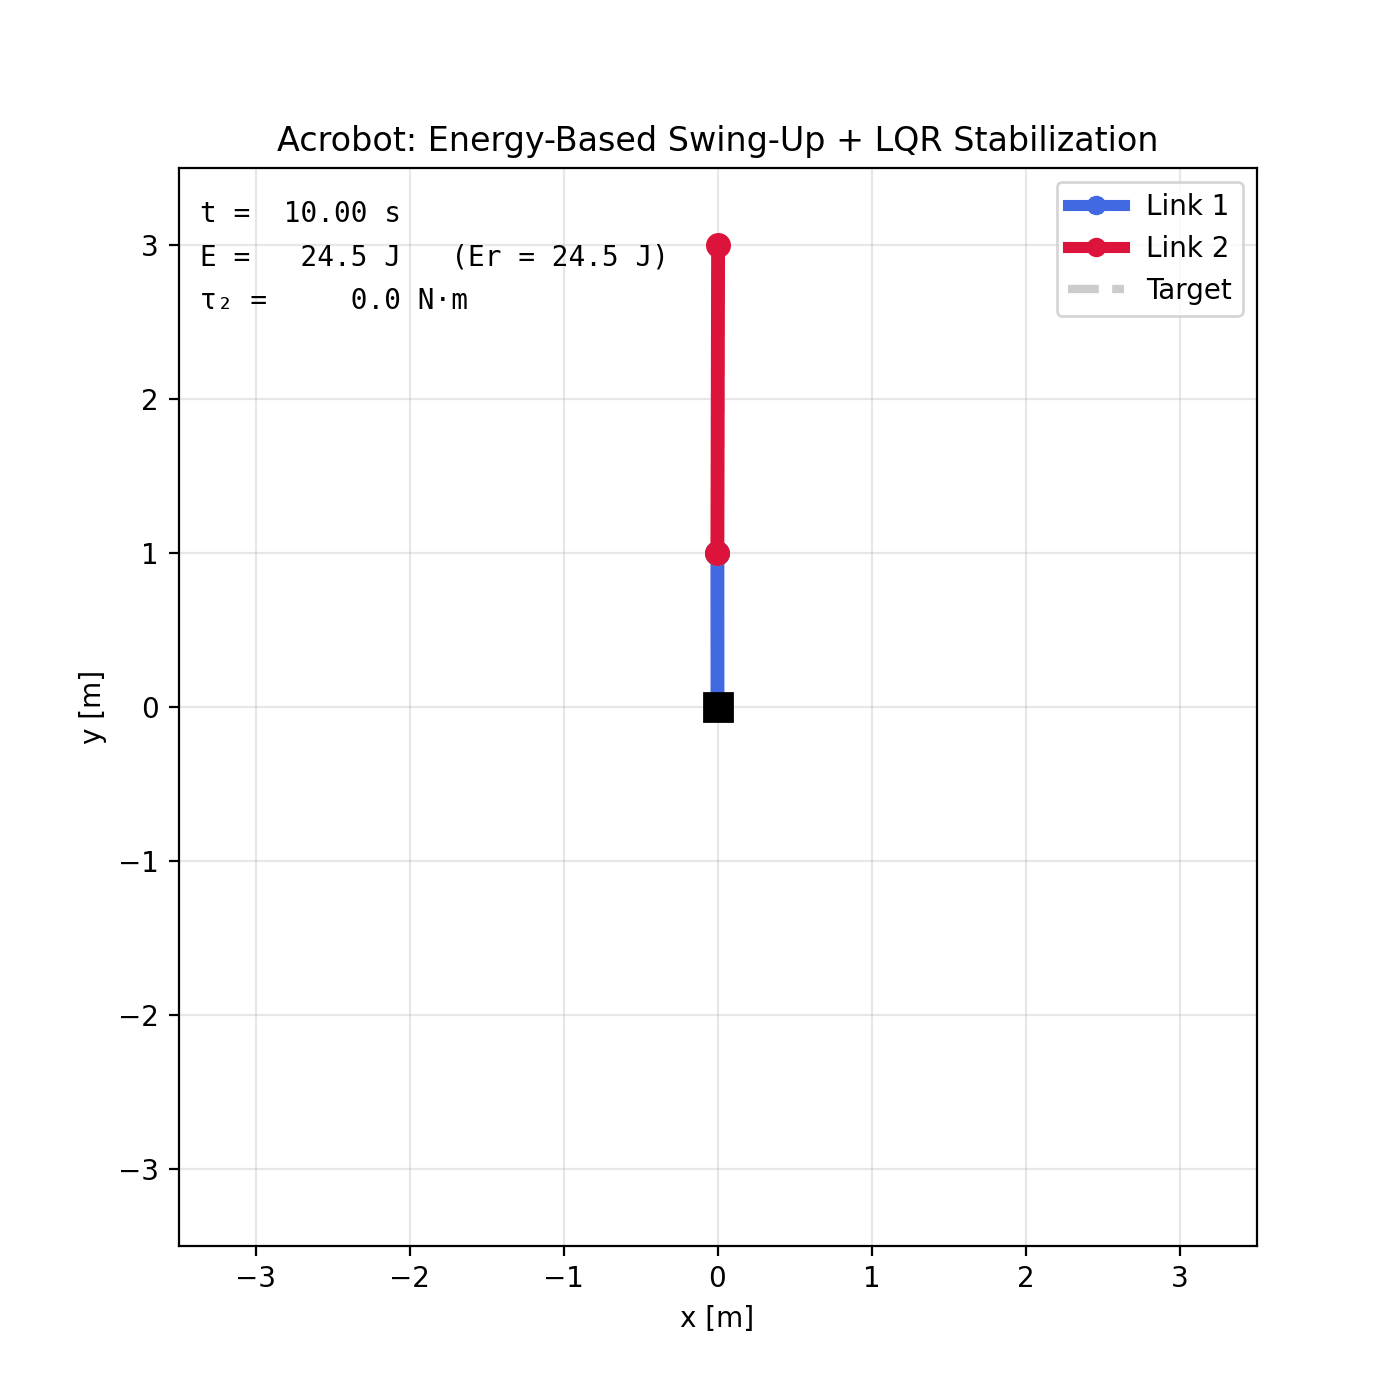
\includegraphics[height=0.78\textheight]{figures/acrobot_frame_swing.png}
\end{frame}
}

\note{%
Here is the animation.
The acrobot starts near the hanging position and swings up.
The backstepping command makes the actuator output track the desired virtual
torque during the swing-up phase.
At about seven point eight seconds, the state enters the LQR region, and the
stabilizer holds it near the upright equilibrium.
}


% =====================================================================
%  SLIDE 9 -- Results: Baseline Comparison
% =====================================================================
\begin{frame}{Results --- Why Backstepping Is Needed}
\begin{columns}[T]
\begin{column}{0.49\textwidth}
  \centering
  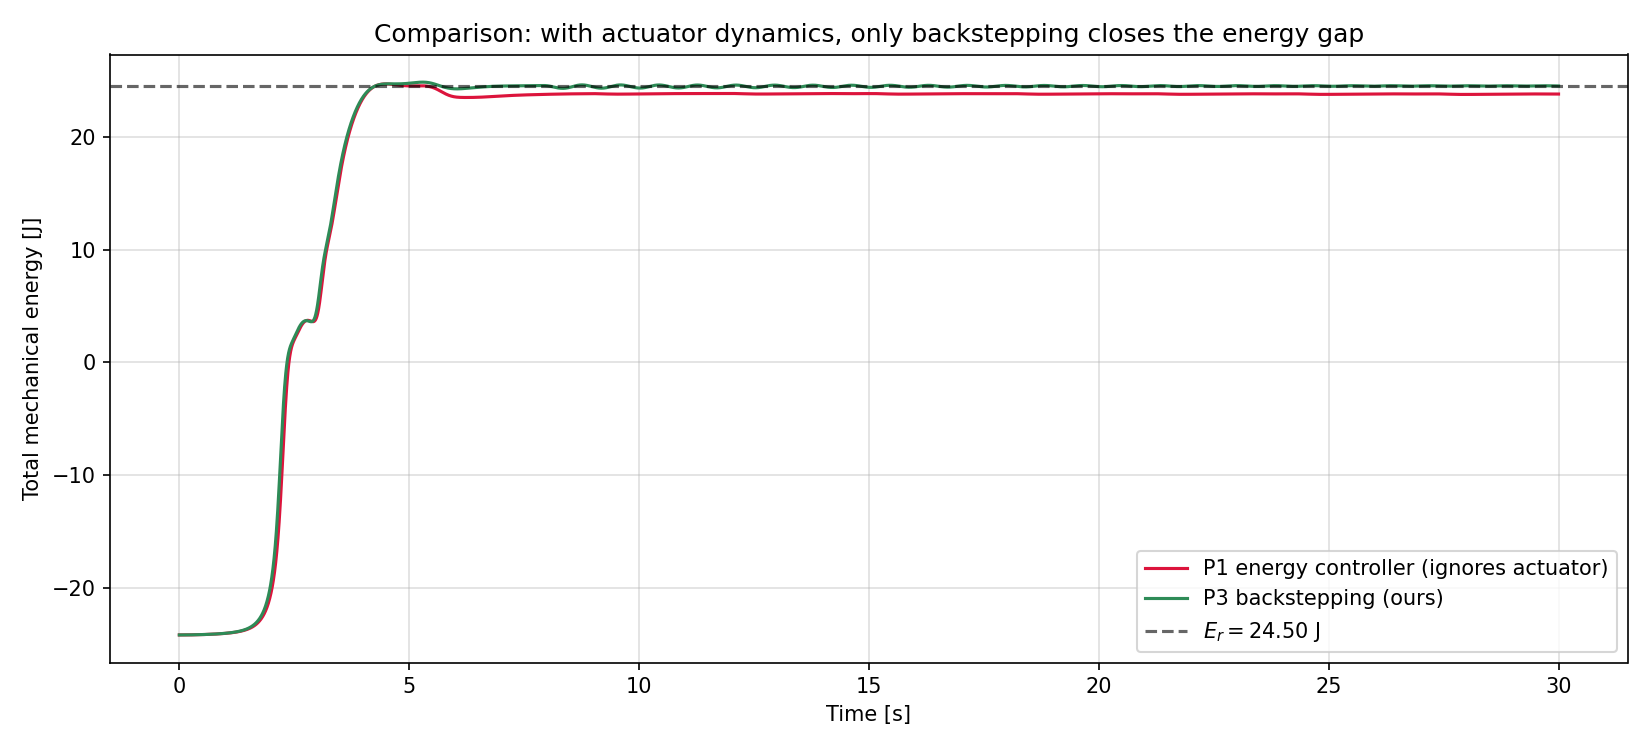
\includegraphics[width=\textwidth]{figures/comparison_energy.png}

  {\small\color{softgray}
  Both controllers pump energy, but the baseline does not settle at the
  upright energy after actuator lag is introduced.}
\end{column}
\begin{column}{0.49\textwidth}
  \centering
  
\includegraphics[width=\textwidth]{figures/comparison_error.png}

  {\small\color{softgray}
  Naive Project~1 control never crosses the $0.04$ switch threshold;
  backstepping enters the LQR basin.}
\end{column}
\end{columns}
\end{frame}

\note{%
These comparison plots show why the extra backstepping loop matters.
The naive Project 1 controller commands the virtual torque directly as u and
ignores actuator lag.

It still injects energy on average, but the lag distorts the pass through the
upright.
The weighted error bottoms out around a few tenths, so the LQR switch never
fires.

With backstepping, the actuator output tracks the virtual control closely, the
trajectory reaches the switch threshold, and LQR can take over.
}


% =====================================================================
%  SLIDE 10 -- Results: Actuator Tracking
% =====================================================================
\begin{frame}{Results --- Actuator Tracking}
  \centering
  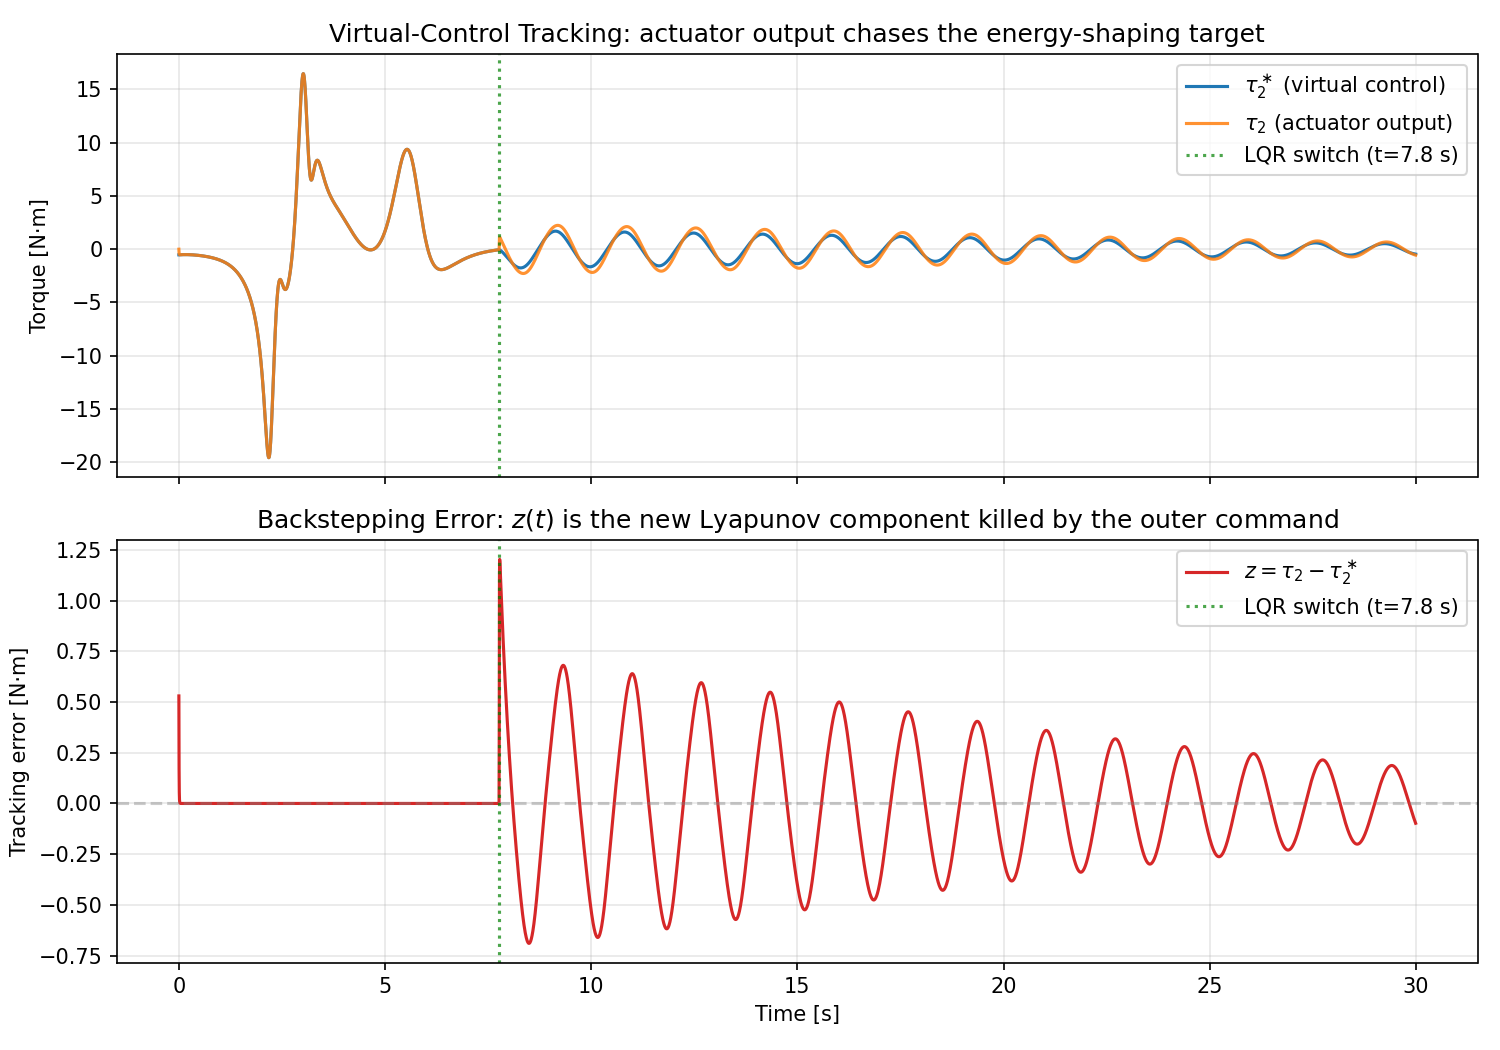
\includegraphics[height=0.69\textheight]{figures/actuator_tracking.png}

  \smallskip
  {\footnotesize\color{softgray}
  The actuator output $\tau_2$ tracks the virtual control $\tau_2^\ast$ during
  swing-up; the visible step marks the handover from backstepping to LQR.}
\end{frame}

\note{%
This is the signature plot for Project 3.
The top panel compares tau-two-star, which is the virtual torque requested by
the outer energy controller, with the actual actuator output tau-two.

The bottom panel shows the tracking error z.
During swing-up, z stays very small, which is exactly what the backstepping
inner loop was designed to do.
}


% =====================================================================
%  SLIDE 11 -- Results: Closed-Loop Response
% =====================================================================
\begin{frame}{Results --- Closed-Loop Response}
\begin{columns}[T]
\begin{column}{0.49\textwidth}
  \centering
  
\includegraphics[width=\textwidth]{figures/tracking_error.png}

  {\small\color{softgray}
  Weighted mechanical error drops after the LQR switch and stays in the
  upright neighborhood.}
\end{column}
\begin{column}{0.49\textwidth}
  \centering
  
\includegraphics[width=\textwidth]{figures/control_signal.png}

  {\small\color{softgray}
  Command $u$ and actuator output $\tau_2$ remain inside the
  $\pm 50$~N\,m saturation limits.}
\end{column}
\end{columns}
\end{frame}

\note{%
The tracking-error plot shows the transition from swing-up to stabilization.
After the switch, the conservative LQR keeps the state close to upright.
It is not as tight as the direct-torque Project 1 result, but it is stable
under the actuator and saturation constraints.

The control plot overlays the command and the actuator output.
They are almost indistinguishable during most of swing-up because the actuator
time constant is small.
}


% =====================================================================
%  SLIDE 12 -- Summary
% =====================================================================
\begin{frame}{Summary}
\footnotesize
\begin{columns}[T]
\begin{column}{0.48\textwidth}
  {\color{okgreen}\textbf{What works:}}
  \begin{itemize}
    \item Backstepping compensates first-order actuator lag
    \item Torque-tracking error decays in ${\sim}4.4$~ms
    \item Swing-up reaches the LQR basin at ${\sim}7.8$~s
    \item Naive Project~1 baseline fails under actuator lag
  \end{itemize}
\end{column}
\begin{column}{0.48\textwidth}
  {\color{warnred}\textbf{Limitations:}}
  \begin{itemize}
    \item Final LQR residual is looser than Project~1
    \item Full 5D LQR gains saturate the command
    \item Larger $T_a$ values need a stronger approach phase
    \item No friction or model uncertainty considered
  \end{itemize}
\end{column}
\end{columns}

\vspace{0.15cm}
\centering
{\large Thank you. We are happy to take questions.}
\end{frame}

\note{%
To summarize: Project 3 takes the energy controller from Project 1 and uses it
as a virtual control inside a backstepping design.
The new inner loop makes the real actuator torque track that virtual torque,
which fixes the actuator-lag failure mode.

The method reaches the LQR basin and stabilizes near upright, while the naive
Project 1 baseline does not switch under the same actuator dynamics.
The main limitations are the conservative LQR residual and the sensitivity to
larger actuator time constants.

Thank you. We are happy to take questions.
}

\end{document}
